The goal of the experiment was to measure the human performance change in a ROV maneuvering task using a predictor display based on image transformation. The participants were given a modified "peg-in-hole" task, where the peg was mounted on a remotely controlled ground vehicle and the holes were rectangular holes in a wooden box.

%A camera was mounted on the ROV such that the operator could see the peg and holes. The goal of the experiment was to measure the operator's navigational performance difference using two different display types. Both displays would use the same fixed delay, but the second would use predictive technology to visualize instant robot responses. The first display would contain a delayed video feed from an ROV while the other display used predictive visualization with the same delay. The participants were given a task of maneuvering the UGV to three specific locations as many times as possible in the course of 90 seconds.

\section{Participants}

The participants were voluntary selected from the NTNU Department of Mechanical and Industrial Engineering. A total of 58 participants performed the experiment whereas the first one were excluded from the data foundation. This was due to lack of information that became evident during the first trial. This information were given to the other $N=57$ participants. None of the subjects had any earlier experience with predictive displays.

33.3\% of the participants were female and the total group had an average age of 24.7 years with an standard deviation (SD) of 1.45. This information among others can be seen in Table \ref{demographicsTable}.
\begin{table}[]
\centering
\vspace*{-2cm}
\caption{Deomgraphic details on participants in experiment.}
\label{demographicsTable}
\small
\begin{tabular}{llllll}
\toprule
                   &                                         & Number of people  & Percentage                              & Mean & SD   \\ \midrule
People tested      & \makecell[lt]{Total\\ Excluded}                       & \makecell[lt]{58\\ 1}           &                                         &      &      \\
Gender             & \makecell[lt]{Male\\ Female}                          & \makecell[lt]{38\\ 19}          & \makecell[lt]{66.7\\ 33.3}                        &      &      \\
Age                &                                         &                   &                                         & 24.7 & 1.45 \\
Use computer daily &                                         & 57                & 100                                   &      &      \\
Gaming             & \makecell[lt]{Daily\\ Weekly\\ Monthly\\ Yearly\\ Never} & \makecell[lt]{2\\ 15\\ 8\\ 17\\ 15} & \makecell[lt]{3.5\\ 26.3\\ 14.0\\ 29.8\\ 26.3} &      &   \\  \bottomrule
\end{tabular}
%\vspace*{-2cm}/
\end{table}

\clearpage
\section{Experimental Design}

\figref{expsetup} shows an overview of the experimental setup. A 17 inch laptop running with a 2.3GHz Intel Core i7-3610QM CPU and Windows 10 together with the arrow keys were used as the operator's control device. This was connected to the ROV through a direct Ethernet connection. 

\begin{figure}[h!]
    \centering
    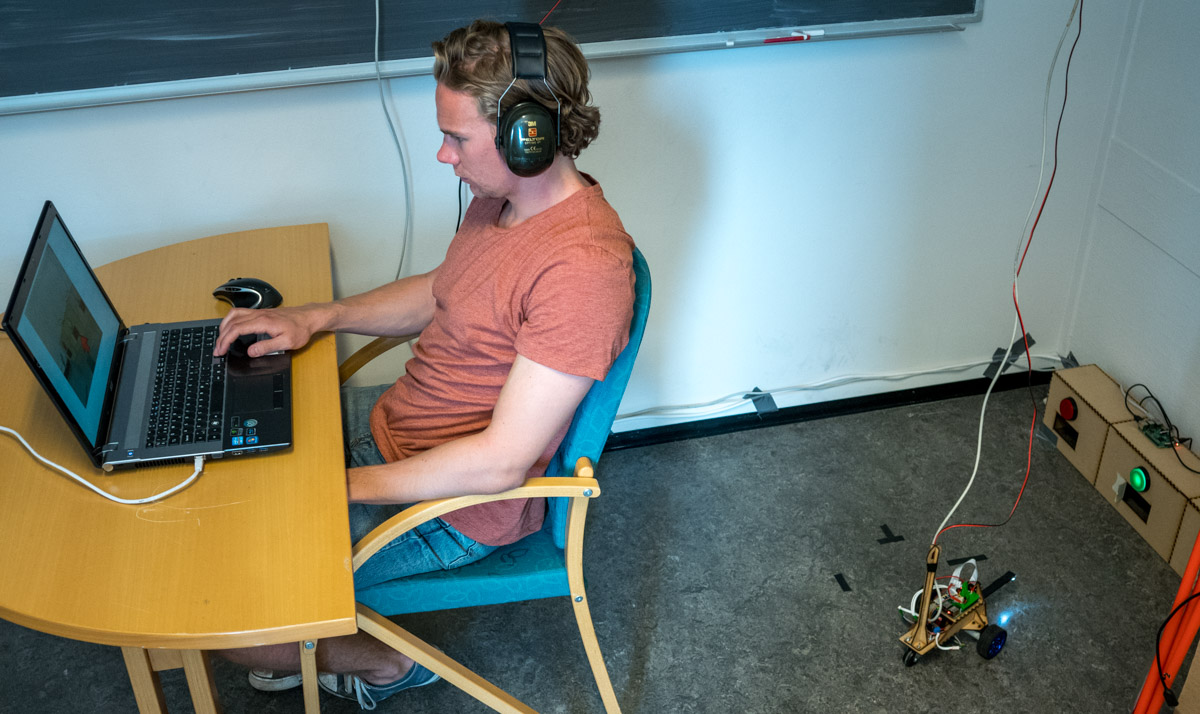
\includegraphics[width=0.8\textwidth]{setup-2}
    \caption{Experimental setup. The computer (left), is used to control the ROV into holes in wooden box (right).}
    \label{expsetup}
\end{figure}

The ROV, \figref{setup3}, was a three wheeled robot running a Raspberry Pi 3 Model B+. Two of the wheels where connected to each their DC-motor while the third one was a caster wheel for support. The ROV was equipped with a forward facing Raspberry Pi Camera V2. The camera has a wide angle lens attached with a horizontal FOV of $76.5$ degrees. The robot was running the eduROV software outlined in chapter \ref{chpEdurov}. This software was responsible for serving the control interface, handling control commands, logging experiment data and adding the desired latency to the communication.

A wooden box with three holes and LEDs were used to register task performance. The distance between the holes (center to center) was $D=30cm$ while the holes itself has a width of $W=10cm$. This translates to a Fitts's \emph{index of difficulty} of $I_d=log_2\left ( 2D/W \right )=2.58\: bits$ \citep{Fitts1954}.

\newgeometry{lmargin=25mm,rmargin=25mm,tmargin=30mm,bmargin=0mm}
\subsection{Task}\label{task}

One by one, in random order, the round LED on the button box would turn on. The operator was then tasked to maneuver the ROV such that the black peg would go inside the corresponding hole. A light sensor inside the hole would register this as a \emph{hit}. This would cause the LED to turn off and one of the other two to turn on. The participants were told to make as many \emph{hits} as possible in the course of 90 seconds.

The participants would repeat this task a total of three times, using three different displays / conditions. The order of these conditions followed a 3x3 Latin Square Design, to eliminate the order effect. Condition one had a total delay of 700 ms which included the inherent system delay of 250ms, plus the added delay of 450 ms. Condition two had the same delay as condition one, but with the predictive display in effect. The third condition had no added delay and only the inherent delay of 250ms. No predictive technology was used in the third condition. The total latency of 700 ms were chosen because it is below the reported threshold for a "move and wait" strategy \citep{Chen2007}, and above what is considered a difficult level in many situations.

\begin{figure}[h!]
    \centering
    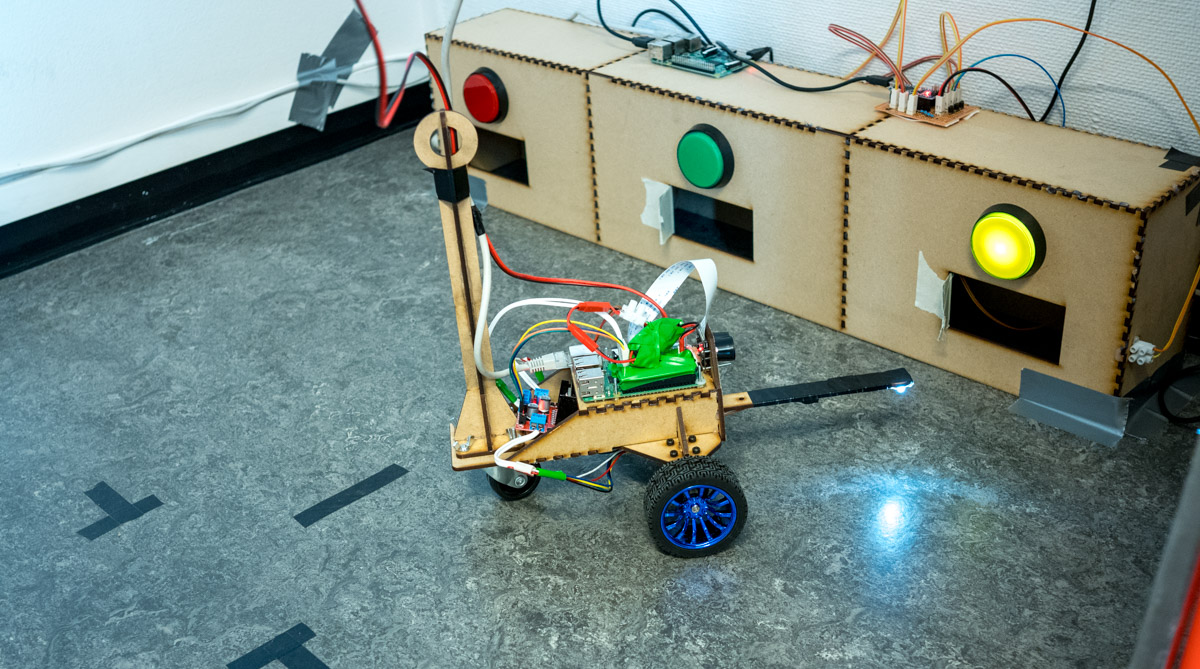
\includegraphics[width=0.65\textwidth]{setup-3}
    \caption{Three wheeled robot used in experiment.}
    \label{setup3}
\end{figure}

Many of the experiments previously mentioned in Table \ref{reviewPred} used a single task and measured the task completion time in different conditions. This experiment was however designed with a single simple task and measured the achieved score in the course of a fixed time period. There are multiple reasons for this choice.
\restoregeometry

First, to reduce the learning effect that would accompany a longer maneuvering course. Some of the authors in Table \ref{reviewPred} reported that the participants performed better for each try when they started to learn the obstacle course. I believe that a longer course would require more time to reduce the learning effect.

Secondly, \citet{Chen2007} reported that the benefit of PD is very task dependent. An easy task was therefore chosen to minimize the effect that task complexity had on the performance results. 

Thirdly, some experiments with real or simulated driving have long stretches with forward motion. The PD provides little help in these situations but still contribute to the task completion time in the same way. A task which required the operator to move from side to side as much as possible was therefore chosen. In addition, by not letting the operator accelerate to maximum ROV velocity, ceiling effects from vehicle limitations were reduced. 

As a fourth argument, a fixed task time made the experiment length much more predictable. Subjects used on average 10 minutes and 56 seconds with a standard deviation of 1 min and 12 seconds to perform the whole experiment. This again made it easier to recruit new subjects. 

As a last argument, the combination of score achievement and time pressure made the subjects fully devoted to the task at hand. This made them performed as close as possible to their potential.

\section{Procedure}

After entering the experiment room, the participants were able to look at the ROV with the button box to get a sense of situational awareness. From that point on, the subject was facing the other way, looking at the computer screen and with the robot outside their FOV. The participants also wore an ear protection headset to remove audible feedback. All the necessary information was given on the screen.

First, the subject S was presented with an initial form collecting demographic data. Then, an information page describing experiment theme, how to steer the robot, the participant's goal and how the experiment would proceed was displayed to the subject. This can be found in \hyperref[appInfo]{Appendix D} on page \pageref{appInfo}. The S was then automatically assigned to a group in correspondence to the 3x3 Latin Square Design. The S then performed a 30 seconds long practice period followed by a 90 seconds long real test. This was done repeatedly for all three conditions. At the end of each test, the S was asked to fill out a test questionnaire.  After each practice and test run, the ROV was repositioned to its original position defined by the black markings in \figref{setup3}. The S was \emph{not} told that one of the conditions would contain a predictor display or how the predictor display worked.

\section{Data Recording and Analysis}

All the data was recorded with the onboard computer of the ROV using a SQLite database. This included demographics, experiment questionnaire data, hits made by the subjects, number of key presses and more. Time stamp data was also recorded for each hit and the test start and end. A total of 11865 data points were collected during the testing period. All the recorded data with exception of the \emph{hits} table is included in \hyperref[appDatabase]{Appendix G} on page \pageref{appDatabase}.

The test questionnaire that was completed for each condition included a NASA TLX (task load index) form \citep{Hart1988}. In addition the S had to guess the total delay that they just experienced. This questionnaire can be found in \hyperref[appSurvey]{Appendix E} on page \pageref{appSurvey}. One modification were done to the NASA TLX form. During the preliminary experiment evaluation, a helper reported that he found it naturally to evaluate a good performance with a high score. In the original questionnaire, a low values translates to a good performance. This metric and the corresponding description was reversed such that a high value would reflect a good performance. After data collection, this value was reversed back such that it can be reported inline with convention.

The number of hits made by the S in the course of 90 seconds was used to quantify performance. This score was normalized in the same way as \citet{Rachmielowski2010} and \citet{Lovi2010} did in their analysis. First, the S's number of hits in a specific condition was divided by the S's average hits achieved in all three conditions. It was then multiplied with the average score for all participants in all conditions. The same normalization has also been done on the reported subjective delay for each condition.

To determine the statistical difference between conditions a two-sided paired sample t-test was used. This was calculated using the \texttt{scipy.stats.ttest\_rel}\footnote{\url{https://docs.scipy.org/doc/scipy/reference/generated/scipy.stats.ttest_rel.html}} function which is a part of the SciPy python library. In the results section, the t-statistics is reported as \emph{t}, the two-tailed p-value as \emph{p} and the degrees of freedom $N-1$ as \emph{df}. A difference is reported as significant if $p\le 0.05$.

When comparing scores based on demographic groups, the variables are no longer dependent. In those cases, a two-sided Welch’s t-test is performed instead. This has been computed using the \texttt{scipy.stats.ttest\_ind}\footnote{\url{https://docs.scipy.org/doc/scipy/reference/generated/scipy.stats.ttest_ind.html}} function. The statistics is reported in the same fashion as in the dependent case, only difference is that the degrees of freedom is calculated using the Welch–Satterthwaite equation \citep{Allwood2008}.

The \emph{effect size}, which describes the magnitude of difference between conditions was calculated using the Cohen's d formula. This value is reported as \emph{d} in the results. When testing for linear relationships between dependent and independent variables, linear least-squares regression is used. It has been calculates using the \texttt{scipy.stats.linregress}\footnote{\url{https://docs.scipy.org/doc/scipy/reference/generated/scipy.stats.linregress.html}} function. The R-squared correlation coefficient is reported as $R^2$.

The code used for the statistical analysis can be found in \hyperref[appAnalysis]{Appendix F} on page \pageref{appAnalysis}.